%!TeX TS-program = Lualatex
%!TeX encoding = UTF-8 Unicode
%!TeX spellcheck = en
%!BIB TS-program = biber
% -*- coding: UTF-8; -*-
% vim: set fenc=utf-8
%%%%%%%%%%%%%%%%%%%%%%%%%%%%%%%%%%%%%%%%%%%%%%%%%%%%%%%%%%%%%%%%%%%%%
\documentclass[11pt]{article}
\usepackage[utf8]{inputenc}
\usepackage{times}
\usepackage{wrapfig}
\usepackage{graphicx}
\usepackage{floatrow}
\usepackage{multicol}
\usepackage{amsmath}

\newcommand{\presynaddr}{a} % pre address
\newcommand{\postsynaddr}{n} % post address
\newcommand{\numevent}{N_{ev}} % total number of events
\newcommand{\presynaddrspace}{\mathcal{A}} %presynaptic address space
\newcommand{\postsynaddrspace}{\mathcal{B}} %postsynaptic address space
\newcommand{\Npol}{N_\text{p}} % number of polarity
\newcommand{\Nneuron}{N_\text{n}} % number of output neurons in the layer
\newcommand{\arank}{r} % address index

\newcommand{\bias}{b} % bias for the MLR model
\newcommand{\synapse}{\sigma} % synapse
\newcommand{\synapticweight}{w} % synaptic weight
\newcommand{\synapticdelay}{\delta} % synaptic delay
\newcommand{\ranksyn}{s} % synapse index
\newcommand{\Nsyn}{N_{s}} % total number of synapses
\newcommand{\activeweights}{\mathcal{W}} 
\newcommand{\timev}{t} % time
\newcommand{\polev}{p} % polarity
\newcommand{\event}{\epsilon} % event
\newcommand{\eventstream}{\xi} % stream of events
\newcommand{\TS}{S} % time surface
\newcommand{\neuron}{\mathbf{n}} % neuron in the SNN (defined by the spatial position and the channel)
\newcommand{\postneuron}{\mathbf{m}} % post synaptic neuron in the SNN (defined by the spatial position and the kernel)
\newcommand{\channel}{\mathbf{p}} % channel
\newcommand{\layer}{\mathbf{L}} % layer
\newcommand{\ms}{\si{\milli\second}}%
\newcommand{\us}{\si{\micro\second}}%
\newcommand{\timecontext}{T} % time context (cf HOTS) matrice gathering last event times
\newcommand{\current}{I} % post synaptic current
\newcommand{\volt}{u} % membrane potential
\newcommand{\mempot}{V} % membrane potential
\newcommand{\restpot}{V_{rest}} % resting membrane potential
\newcommand{\threspot}{V_\theta} % membrane potential threshold
\newcommand{\gain}{\gamma} % homeostatic gain
\newcommand{\simil}{\beta} % similarity value
\newcommand{\Nclass}{N_\text{class}} % number of classes for MLR:
\newcommand{\Nx}{N_\text{X}}
\newcommand{\Ny}{N_\text{Y}}
\newcommand{\Ntime}{N_\text{t}}
\newcommand{\kernel}{K} % convolution kernel
%\newcommand{\kernelind}{\mathbf{k}} % indice of the kernel
\newcommand{\kernelind}{k} % indice of the kernel
\newcommand{\Kx}{K_\text{x}}
\newcommand{\Ky}{K_\text{y}}
\newcommand{\Ktime}{K_\text{t}}
\newcommand{\classiflayer}{\mathbf{C}}
\newcommand{\class}{c} % class k of the MLR
\newcommand{\lrweights}{\theta} % matrix of MLR weights
\newcommand{\lrtrue}{y} % true value of the prediction for MLR
\newcommand{\loss}{\mathcal{L}} % cost function for MLR
\newcommand{\softmax}{\sigma}
\newcommand{\firerank}{f}
\newcommand{\decision}{\hat{y}}
\newcommand{\speed}{v}
\newcommand{\Nspeed}{N_v}
\newcommand{\colorsec}{red}
\newcommand{\colorsubsec}{gray}
\newcommand{\learningrate}{\mu}



\oddsidemargin -0.5in		% margin, in addition to 1" standard
\textwidth 7.5in		% 8.5" - 2*(1+\oddsidemargin)

\topmargin -1in		% in addition to 1.5" standard margin
\textheight 9.75in 		% 11 - ( 1.5 + \topmargin + <bottom-margin> )

\columnsep 0.25in

\parindent 0pt
\parskip 12pt

\flushbottom \sloppy
\pagestyle{empty} % No page numbers
%%%%%%%%%%%%%%%%%%%%%%%%%%%%%%%%%%%%%%%%%%%%%%%%%%%%%%%%%%%%%%%%%%%%%
\usepackage[
%style=chem-acs,
style=numeric,						% numeric style for reference list
citestyle=numeric-comp,
%style=alphabetic-verb,
giveninits=false,
maxbibnames=1,
%firstinits=true,
%style=apa,
%maxcitenames=1,
%maxnames=3,
%minnames=1,
%maxbibnames=99,
dateabbrev=true,
giveninits=true,
%uniquename=init,
url=false,
doi=false,
isbn=false,
eprint=false,
texencoding=utf8,
bibencoding=utf8,
autocite=superscript,
backend=biber,
%sorting=none,
sorting=none,
sortcites=false,
%articletitle=false
]{biblatex}%

\bibliography{ref.bib}
%%%%%%%%%%%%%%%%%%%%%%%%%%%%%%%%%%%%%%%%%%%%%%%%%%%%%%%%%%%%%%%%%%%%%%
\newcommand{\mycaption}[1]{\caption*{#1}}

\usepackage{titlesec}
% \titlespacing*{<command>}{<left>}{<before-sep>}{<after-sep>}
\titlespacing*{\section}
{0pt}{1.5ex}{0.8ex}
\titlespacing*{\subsection}
{0pt}{0.9ex}{0.4ex}
\titlespacing*{\subsubsection}
{0pt}{0.5ex}{0.3ex}
\titlespacing*{\paragraph}{%
  0pt}{%              left margin
  0.0\baselineskip}{% space before (vertical)
  1em}%               space after (horizontal)

\usepackage{setspace}

\begin{document}

%%%-----------------------------------------------------------------
{\Large\bf %Unsupervised learning of precise spiking motifs with a heterogeneous synaptic delays neuron model
Unsupervised learning of a precise spiking motif using a STDP on weights and delays
}\\

%{\bf
%Anonymous submission for double-blind review. \\
%}
\hrule
%%SUMMARY
%%%-----------------------------------------------------------------
\textbf{Summary} %}
The spiking response of a biological neuron depends on the precise timing of afferent spikes and this temporal aspect of the neuronal code is essential in understanding information processing in neurobiology. In particular, it was shown that introducing heterogeneous synaptic delays in spiking neuron models allows them to become selective to precise spiking motifs. Indeed, the variety of synaptic delays on the dendritic tree allows synchronizing synaptic inputs as they converge on the soma of the neuron. In this study, we propose a bio-plausible unsupervised learning rule on both weights and delays through the derivation of a loss function which depends on the membrane potential of the spiking neuron. These models can learn spiking motifs only with supervised Spike-Timing Dependent Plasticity (STDP) rules based on the desired output spike. This gradient-based approach maximizes the membrane potential of the neuron at the timing of the output spike. We add a regularization term to the loss function, formalizing a homeostatic mechanism on the spiking activity of neurons: Their gain can be increased or decreased according to a target firing rate, with no supervision on the output spike time. We demonstrate, on synthetic data, that such spiking neuron is able to learn a precise spatio-temporal motif embedded in the spike train. This original and simple learning rule can be applied to a layer of neurons with a winner-take all mechanism in order to learn multiple spiking motifs. We aim at generalizing this detection to neurobiological data. %Results show a large improvement in performances when adding temporal delays for computations and a great increase in robustness to noise.
\vspace{.5cm}
\hrule
%---------------------------

\begin{wrapfigure}{R}{.7\textwidth}
\vspace{-15pt}
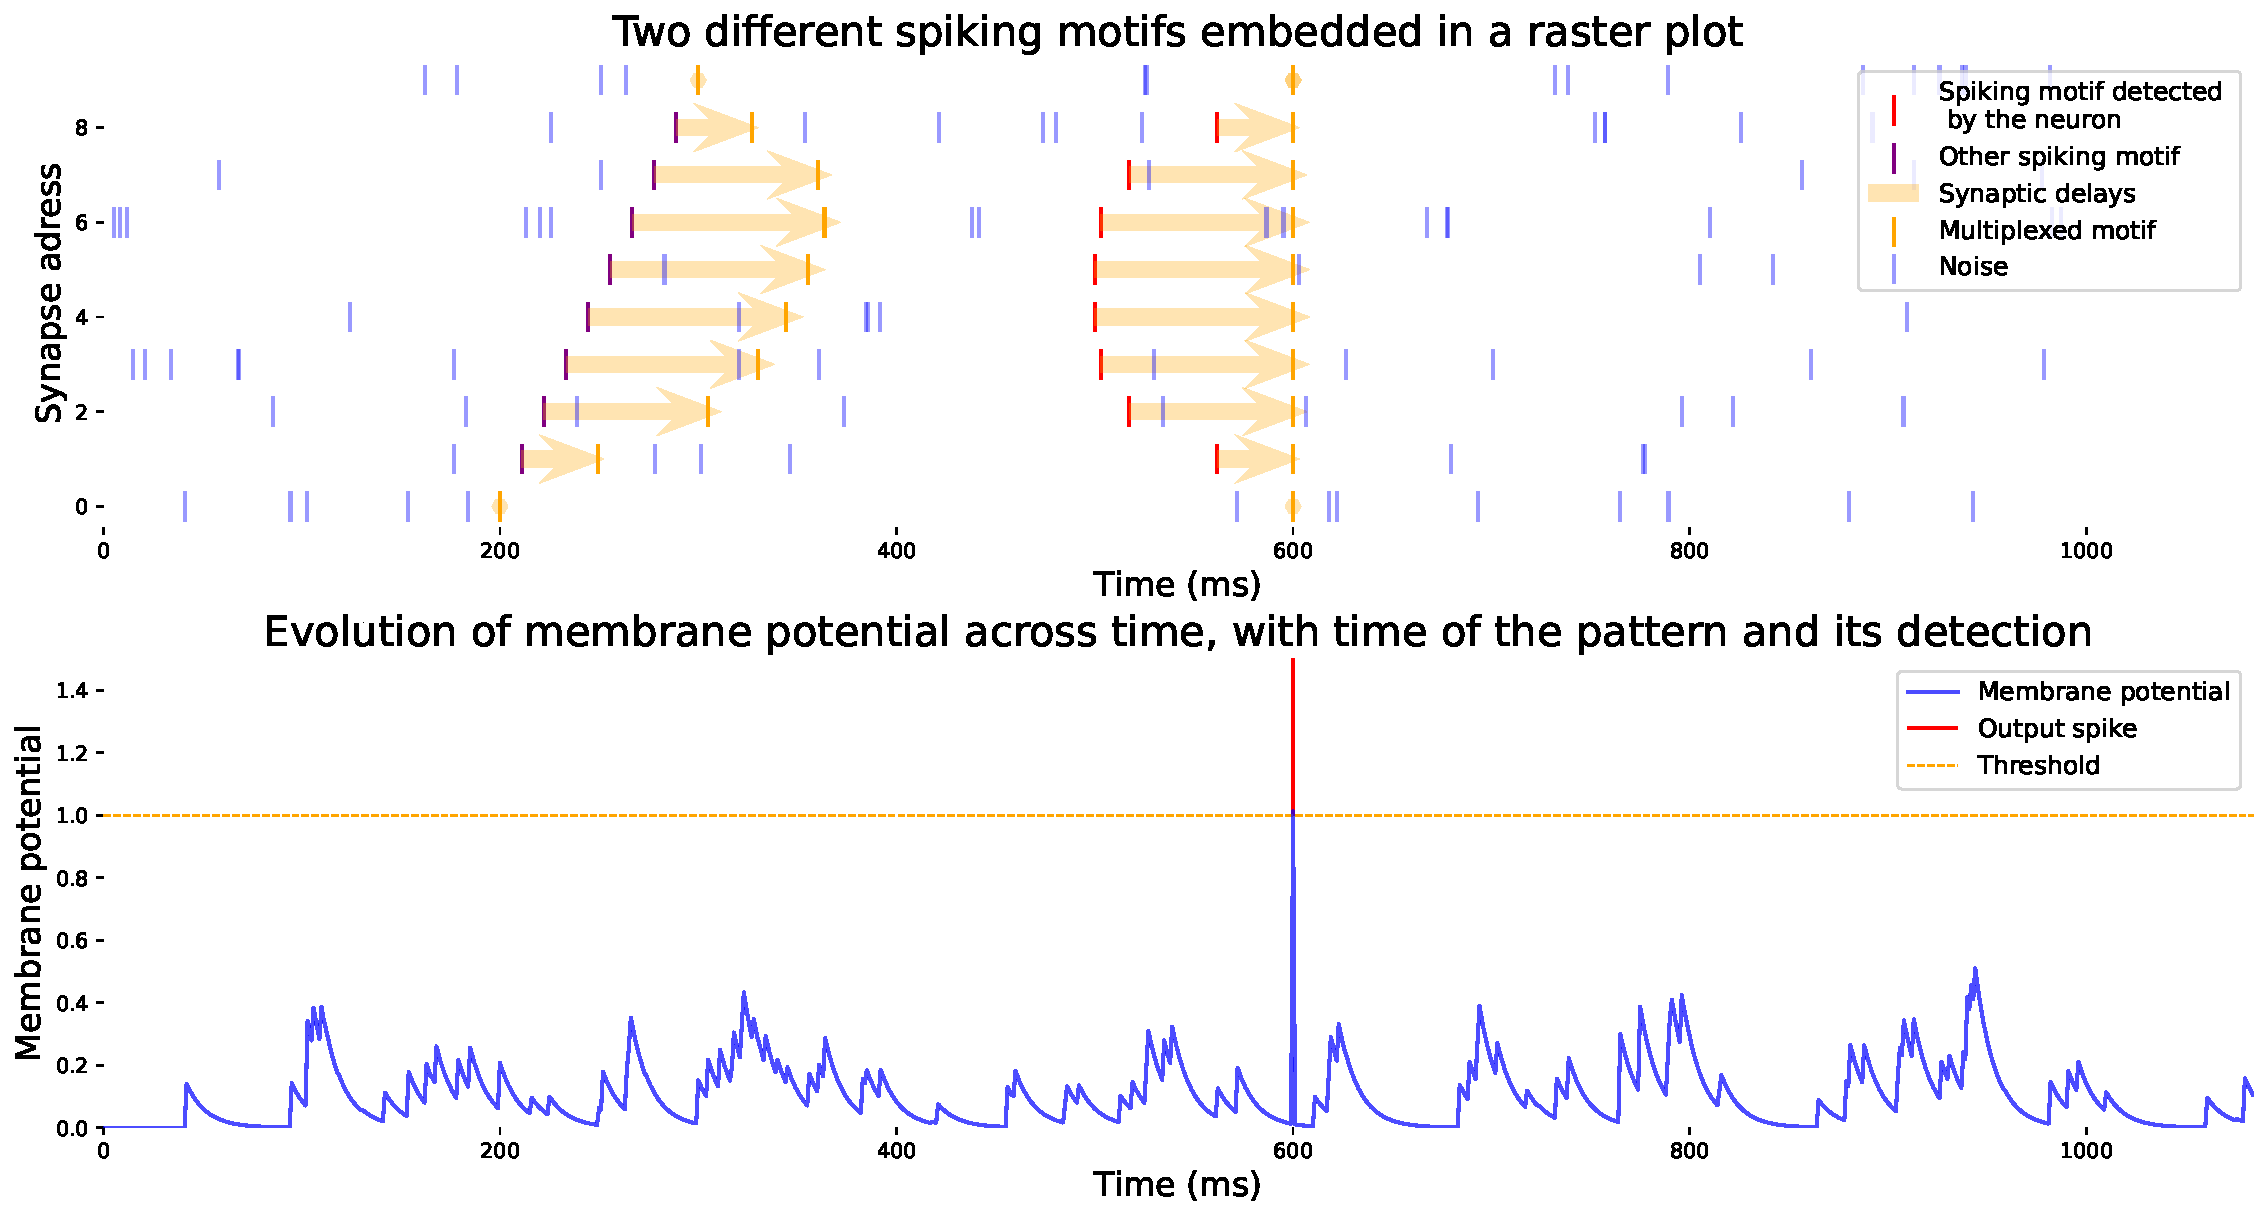
\includegraphics[width=0.99\linewidth]{heterogeneous_neuron.pdf}
\vspace{-25pt}
\end{wrapfigure}

%---------------------------
\textbf{Additional Details.}%
%
% * Limit : not online - in the future it is a model of a neuron
%
\paragraph*{Figure 1 (right): Heterogeneous delays neuron model for spiking motif detection}

Given a generic raster plot defined by a set of spikes occurring on specific addresses and at specific times, one may consider that this information consists in the repeated occurrence of groups of precise motifs of spikes. The top part of the figures represents a raster plot with the occurrence of 2 different spiking motifs: a purple one and a red one. The orange arrows represent the synaptic delays (the longer the arrow, the longer the delay) of our spiking neuron model that will multiplex in time the incoming spikes. Multiplexed patterns are drawn in orange and represent the time at which incoming spikes will reach the soma of the neuron. One can notice that spikes from the red pattern will reach the soma synchronously. The bottom part of the figure represent the evolution of the membrane potential of the spiking neuron. At 600 ms, all spikes from the red spiking motif reach the soma at the same time leading to a sudden increase of the membrane potential on the neuron. Note that the neuron is not very sensitive to the background activity or the other spiking motif, only this synchronous arrival of the red spikes leads to an output spike represented in red on the bottom figure. The spiking mechanism of this neuron acts as a coincidence detector on the postsynaptic activity. A mathematical formulation is given by equation~\eqref{eq:mem_pot}. 

\paragraph*{Mathematical formalism of the membrane potential of our spiking neuron model:}
\begin{equation}
\mempot(\timev) = \restpot + \gain \cdot (\threspot-\restpot) \cdot \sum_{\ranksyn} \synapticweight_\ranksyn \sum_{\arank \in \eventstream_\ranksyn} \kernel_\ranksyn(\timev, t_\arank) - \sum_{\firerank \in \eventstream_\channel} (\threspot-\restpot) \cdot e^{-\frac{\timev - \timev_\firerank}{\tau}}
\label{eq:mem_pot}
\end{equation}
where $\restpot$ is the resting membrane potential, $\threspot$ is the membrane potential threshold, $\synapticweight_\ranksyn$ and $\synapticdelay_\ranksyn$ are respectively the synaptic weight and delay of synapse $\ranksyn$, $\gain$ is the gain of the neuron, $\eventstream_\ranksyn$ and $\eventstream_\channel$ are both event streams associated respectively to the synaptic address $\ranksyn$ and the neuronal address $\channel$ and $\kernel_\ranksyn$ is the kernel applied to the input spikes. Note that this formulation corresponds to the solution of a Leaky Integrate and Fire (LIF) neuron if we use the following kernel: $\kernel_\ranksyn(\timev, \timev_\arank) = e^{-\frac{ \timev-\timev_\arank-\synapticdelay_\ranksyn}{\tau}}$.\\
\\
\break
%
\vspace{-1.5cm}
\paragraph*{Unsupervised learning\\}

\begin{multicols}{2}

We report few existing methods using the proposed spiking mechanism and training synaptic weights and delays~\cite{nadafian_bio-plausible_2020, zhang_supervised_2020}. However, \cite{nadafian_bio-plausible_2020} does not converge and needs a stop condition on the delay learning and~\cite{zhang_supervised_2020} is supervised on the desired postsynaptic spike time. 
Here, we propose a generic gradient-based learning rule on both weights and delays. 
We define a loss function (equation~\eqref{eq:loss}) that will maximize the membrane potential of the neuron at the output spike time ($\timev_\firerank$). Delays will be adjusted to synchronize the repeating spiking motifs (equation~\eqref{eq:delay}) and weights will be increased when the corresponding delays match correctly the input spikes (equation~\eqref{eq:weight}). Because synaptic weights are normalized to sum to 1, they will represent the probability of the associated presynaptic neuron to contribute to the spiking motif. Then, patterns do not have to be composed of the same number of spikes. A regularization term is added to keep a stable firing rate ($r_\channel$) for the neuron (right term of equation~\eqref{eq:loss}). The gain of the neuron can be adjusted to respect this condition. From this loss function, we can derive learning rules for both synaptic weights and delays, and a homeostatic regulation rule, of the neuron. We can this generic formulation to different types of kernel to model the postsynaptic activity. In this work, we choose a non-causal LIF kernel (equation~\eqref{eq:nclk}). It can also be generalized for a layer of neurons with a winner-take-all mechanism to detect multiple spiking motifs.

\columnbreak
\noindent \textbf{Loss function:}
%
\begin{equation}\label{eq:loss}
\loss(\timev_\firerank) = -\mempot(\timev_\firerank) + \lambda \cdot \left| N_\firerank - r_\channel \cdot T \right|
\end{equation}
$\lambda$ is a regularization factor, $N_\firerank$ is the number of spikes that occured during time window $T$ and $r_\channel$ is the objective average firing rate for neuron $\channel$.\\
%
\\
\textbf{Learning rule for the delays and the weights:}
%
\begin{equation}\label{eq:delay}
\synapticdelay_\ranksyn = \synapticdelay_\ranksyn + \learningrate_\synapticdelay \cdot \synapticweight_\ranksyn \cdot \sum_{\arank \in \eventstream_\ranksyn} \frac{\partial \kernel_\ranksyn(\timev_\firerank, t_\arank)}{\partial \synapticdelay_\ranksyn}
\end{equation}
%
\begin{equation}\label{eq:weight}
\synapticweight_\ranksyn = \synapticweight_\ranksyn + \learningrate_\synapticweight \cdot \sum_{\arank \in \eventstream_\ranksyn} \kernel_\ranksyn(\timev_\firerank, t_\arank)
\end{equation}
\\
\textbf{Homeostatic adaptation of the gain:}
\begin{equation}\label{eq:gain}
\gain = \gain + \learningrate_\gain \cdot \lambda \cdot N_\firerank \cdot sgn(1-\gain)/T
\end{equation}

For this work, we use a non causal LIF kernel for the training:
\begin{equation}\label{eq:nclk}
\kernel_\ranksyn(\timev_\firerank, \timev_\arank) = e^{-\frac{\left| \timev_\firerank-\timev_\arank-\synapticdelay_\ranksyn \right|}{\tau}}
\end{equation}
$$\frac{\partial \mempot(\timev_\firerank)}{\partial \synapticdelay_\ranksyn} = \frac{\synapticweight_\ranksyn}{\tau} \sum_{\arank \in \eventstream_\ranksyn}sgn(\timev_\firerank-\timev_\arank-\synapticdelay_\ranksyn) \cdot \kernel_\ranksyn(\timev_\firerank, \timev_\arank)$$
\end{multicols}
%

\paragraph*{Figure 2}
Here put a figure where we learn different types of spiking motifs with one neuron

Maybe add a figure where we show the STDP with the delays and the evolution of the weights as well
%
\printbibliography
\end{document}
